%
%                       This is a basic LaTeX Template
%                       for the Informatics Research Review

\documentclass[a4paper,11pt]{article}
% Add local fullpage and head macros
\usepackage{head,fullpage}     
% Add graphicx package with pdf flag (must use pdflatex)
\usepackage[pdftex]{graphicx}  
% Better support for URLs
\usepackage{url}
% Date formating
\usepackage{datetime}
% For Gantt chart
\usepackage{pgfgantt}
\usepackage{xcolor}
\usepackage[utf8]{inputenc}
\usepackage{subcaption}

\newdateformat{monthyeardate}{%
  \monthname[\THEMONTH] \THEYEAR}

\parindent=0pt          %  Switch off indent of paragraphs 
\parskip=5pt            %  Put 5pt between each paragraph  
\Urlmuskip=0mu plus 1mu %  Better line breaks for URLs


%                       This section generates a title page
%                       Edit only the following three lines
%                       providing your exam number, 
%                       the general field of study you are considering
%                       for your review, and name of IRR tutor

\newcommand{\examnumber}{B240710}
\newcommand{\field}{Leveraging Bipartite Network of Investor-Startup Ecosystem for Predicting Startup Growth and Success}
\newcommand{\tutor}{Felipe Costa Sperb}
\newcommand{\supervisor}{Valerio Restocchi}

\begin{document}
\begin{minipage}[b]{110mm}
        {\Huge\bf School of Informatics
        \vspace*{17mm}}
\end{minipage}
\hfill
\begin{minipage}[t]{40mm}               
        \makebox[40mm]{
        \includegraphics[width=40mm]{crest.png}}
\end{minipage}
\par\noindent
    % Centre Title, and name
\vspace*{2cm}
\begin{center}
        \Large\bf Research Methods in Financial Computing \\
        \Large\bf \field
\end{center}
\vspace*{1.5cm}
\begin{center}
        \bf \examnumber\\
        \monthyeardate\today
\end{center}
\vspace*{5mm}

%
%                       Insert your abstract HERE
%                       
\begin{abstract}
This research proposes to utilize network science to analyze a bipartite network comprising investors and start-ups. By employing methodologies such as centrality analysis and community detection, we aim to map the intricate relationships between investors and start-ups and predict future growth trajectories and success rates. The nodes in this network will represent both investors and start-ups, while links will denote investment relationships. This will represent the investor-start-up dynamics that influence start-up outcomes. This will offer venture capital firms and entrepreneurs a strategic tool to make informed decisions and optimize their investment and growth strategies, fostering robust entrepreneurial ecosystems.
\end{abstract}

\vspace*{1cm}

\vspace*{3cm}
Date: \today

\vfill
{\bf Tutor:} \tutor\\
{\bf Supervisor:} \supervisor
\newpage

%                                               Through page and setup 
%                                               fancy headings
\setcounter{page}{1}                            % Set page number to 1
\footruleheight{1pt}
\headruleheight{1pt}
\lfoot{\small School of Informatics}
\lhead{Informatics Research Review}
\rhead{- \thepage}
\cfoot{}
\rfoot{Date: \date{\today}}
%


\section{Motivation}
In the rapidly evolving landscape of technological innovation and entrepreneurship, the capacity to predict and foster start-up success is crucial not only for individual companies but also for investors. With almost five million new start-ups were created in 2022 alone based on Embroker Analysis \cite{embroker2024a}, the relationships between investors and start-ups grow ever more complex. They naturally create a web of relationships that can significantly impact a startup’s access to resources, market entry, and competitive positioning. Therefore, according to Uzzi, the position
a start-up within its ecosystem is relevant for its future success \cite{uzzi2021a}.

This research will delve into the application of network science to untangle this complexity by building and analyzing a bipartite network that includes both investors and start-ups (will later be referred to as an investor network in this proposal). Particularly, the methodologies of centrality analysis and community detection will serve to illuminate the patterns of interaction that are most conducive to successful innovation ecosystems. By representing both investors and startups as nodes and their financial engagements as links, this study will provide a structural and dynamic view of the investment landscape.

The scope of this research encompasses the construction of this network, the application of aforementioned analytical methodologies to discern key patterns, and the prediction of future growth trajectories and success of start-ups based on their network positions. This approach will refine the strategies employed by venture capitalists and entrepreneurs alike, offering them a more nuanced tool for decision-making than currently available methods, such as financial metrics analytics \cite{gompers2016a}.

\subsection{Problem Statement}
Despite the critical role of investor in the startup ecosystem and abundant data on investment amounts and funding rounds, there remains a significant gap in understanding how the specific structures and characteristics of these investor networks influence startup outcomes. Most current models focus predominantly on utilization of machine learning \cite{krishna2016a} \cite{carniel2023a} \cite{sharchilev2018a} \cite{yang2020a}, overlooking the broader network characteristics that can significantly influence startup success and lacking explainability. This gap presents a critical area for exploration, particularly given the lack of a more nuanced, predictive framework that incorporates the intricate web of relationships and interactions within the start-up investment landscape.

This research will aim to answer the question: How do the connectivity and characteristics of investor networks affect the growth trajectories and success of startups? By limiting the investigation to these network characteristics, the research will try to provide a more nuanced understanding of how investor relationships within these networks directly correlate with startup growth and sustainability, thereby offering an additional foundational tool for strategic decision-making in the investment community.

\subsection{Research Hypothesis and Objectives}
This research will investigate the hypothesis that the connectivity and characteristics of investor networks, specifically the centrality measures of investors and the structure of investment communities, significantly influence the growth trajectories and success of startups. We hypothesize that startups linked to highly central investors within cohesive investment communities will likely demonstrate higher growth rates and chance of success. This will align with the previously mentioned theory that the position of a start-up within its ecosystem is relevant for its future success, as the relationships within the ecosystem itself dictate access to resources, knowledge, and opportunities \cite{uzzi2021a}.

There are four objectives in this research. 
\begin{itemize}
    \item Construct a comprehensive network model of investor-startup relationships that incorporates quantitative investment data
    \item Analyze the centrality of investors within the network to assess how these measures correlate with the success metrics of funded startups
    \item Identify and analyze the structure of communities within the investor network to determine their impact on startup outcomes
    \item Examine the evolution of the investor-startup network over time, capturing dynamic changes and their effects on startup growth and success
\end{itemize}

This research will not explore the qualitative aspects of investor-startup relationships, such as the quality of mentorship or the level of investor involvement, beyond their quantifiable impact through network structures. Furthermore, the focus will be primarily on quantifiable network metrics and their direct correlations, rather than on external factors like market conditions or technological innovations that could also significantly impact startup success.

\subsection{Timeliness and Novelty}

The proposed research is exceptionally timely given the current global economic landscape, characterized by rapid technological advancements and an increasingly competitive startup ecosystem. Venture capital firms and entrepreneurs are in constant search of innovative tools that provide a competitive edge in identifying and nurturing potential successful ventures. As the total venture capital funding reached a decade-high of 200 billion dollar in 2022 \cite{embroker2024a} with only half of the invested companies survive until their fifth year \cite{kotashev2024a}, the opportunity to leverage this data through network science for predictive analytics is more pertinent than ever.

The novelty of this research is highlighted by its innovative approach to constructing a bipartite network analysis that integrates both investors and startups, specifically aimed at predicting venture capital success and startup growth. This is a significant departure from existing research, which predominantly focuses on machine learning techniques \cite{krishna2016a} \cite{sharchilev2018a}, hybrid network science and machine learning techniques \cite{carniel2023a} \cite{yang2020a}, agent based modeling \cite{lengyel2020a}, and qualitative analysis \cite{mccarthy2023a}. Moreover, even in instances where non-hybrid network science is considered, the created networks typically revolve around other characteristics such as employee \cite{bonaventura2020a}. By shifting the focus to a bipartite network and applying network science methodologies like centrality analysis and community detection, this research will offer a new perspective and toolkit for understanding and leveraging the dynamics of investor influence on startup success, filling a crucial gap in current academic and practical approaches to predict startup growth and success.

\subsection{Significance}

This research innovates by transitioning from traditional financial metrics to a network analysis approach, providing a more holistic view of the startup ecosystem. By focusing on relationships and network positions, it will identify key dynamics and environmental influences that are crucial for startup success, moving beyond mere financial indicators. The use of centrality and community detection techniques will allow for the identification and explanation of influential entities within the network, something that machine learning techniques are lacking. Furthermore, it will try to offer a new horizon of understanding by integrating investor relationships as an additional layer of analysis. This will not only complement the existing focus on other relationships, but also allow for a more comprehensive prediction model that captures both the human capital and financial investment aspects of startup ecosystems, leading to more accurate forecasts and more informed decision-making in the venture capital sector.

The immediate applications of this research are substantial. For venture capital firms, the findings can lead to more informed and strategic investment decisions, potentially increasing the success rate of their portfolios. For startups, insights from this study can guide strategies for networking and securing investment, directly impacting their growth trajectories. Further research based on the findings of this study could explore longitudinal impacts of network changes, delve deeper into the causal relationships between network position and startup success, or expand the network analysis to include other characteristics such as location, customers, and founders. Each of these avenues not only broadens the scope of network analysis but also enhances our collective ability to foster robust, sustainable entrepreneurial environments. This research not only fills a current gap but sets the stage for a deeper, more comprehensive exploration of the factors driving startup success.

\subsection{Feasibility}

The feasibility of this research will be grounded in the practicality of its methodology and the accessibility of its primary data source, the Crunchbase Application Programming Interface (API), which provides a comprehensive and continuously updated dataset of startups, investors, and investment transactions. This data richness and availability significantly enhance the feasibility of conducting extensive network analyses within a constrained timeframe and with limited resources.

To ensure the study's feasibility before proceeding with major implementation work, a preliminary feasibility study will be conducted. This will involve:
\begin{itemize}
    \item Initial tests will be run on the Crunchbase API to confirm the availability and integrity of the data required for the study, particularly regarding investor-startup relationships and investment details. This will help identify any potential data gaps or limitations in the API's scope
    \item An evaluation of the computational resources needed to process and analyze the data will be undertaken. This includes assessing the software and hardware requirements for handling large datasets and complex network analyses, ensuring that the necessary tools and capacities are in place
    \item A detailed timeline will be developed, outlining key milestones and deliverables. This will ensure that the research remains on track and within the allocated time, addressing potential bottlenecks or delays early in the process. Please find the detail in section 6
\end{itemize}

By addressing these key aspects, we can minimize risks and ensuring that the study can be conducted effectively within its constraints. This preparatory phase is critical to guarantee that the full research is practical, achievable, and capable of producing valuable insights within the limited timeframe and resources available.

\subsection{Beneficiaries}

This research is poised to benefit a wide range of stakeholders, particularly researchers in the fields of economic sociology, business studies, and data science, by providing a deeper understanding of how investor networks influence startup success. The findings will offer valuable insights into network effects and social capital, broadening the academic discourse around these topics and contributing to more nuanced theories in these areas. To ensure that these benefits are accessible, the research outcomes will be disseminated through multiple channels. Key findings will be submitted to peer-reviewed journals, ensuring rigorous review and wide academic reach. This will facilitate knowledge sharing and potentially inspire further research based on the findings. To enhance accessibility and foster further academic work, all datasets processed and analyzed during the study, subject to privacy and confidentiality constraints, will be made available in a public repository. Moreover, detailed methodologies and tools developed will be documented and published in open-access formats, allowing other researchers to replicate or build upon this work. Through these efforts, the research will aim to not only advance understanding within its specific area but also support interdisciplinary work that intersects with network analysis, startup dynamics, and investment strategies.

\section{Background and Related Work}

This section provides the definitions for the most important concept used in the proposed research. There are several key concepts in our research, which include:

\textbf{Bipartite Network}: A type of graph in network science where nodes are divided into two disjoint sets, and edges can only connect nodes from different sets \cite{guillaume2005a}. In this study, one set represents startups and the other represents investors, with edges signifying investment relationships. The example of Bipartite Network can be seen in Figure 1 below.

\begin{figure}[h]
\centering
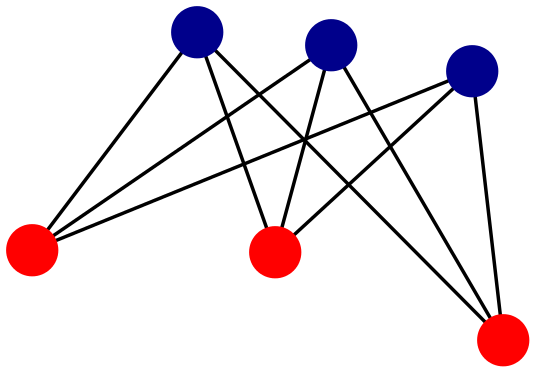
\includegraphics[width=0.25\textwidth]{bipartite.png}
\caption{Bipartite Network}
\end{figure}

\textbf{Centrality Analysis}: A method used to identify the most influential nodes within a network based on their position \cite{albert2019a}. In this proposed research, this involves quantifying how central a startup or investor is within the bipartite network, which is crucial for understanding their potential impact on the network’s dynamics and outcomes. We will use both degree centrality and closeness centrality to do the analysis. Degree centrality is the simplest form of centrality and measures the number of direct connections a node has. In our network, it can help identify investors who are heavily investing across various startups or startups that are attracting numerous investors. On the other hand closeness centrality reflects how close a node is to all other nodes in the network, providing insights into how quickly information from the node can spread throughout the network. Investors with high closeness centrality can affect the startup ecosystem more rapidly than others. To better understand the definition of these two types of centrality, please take a look into Figure 2 below.

\begin{figure}[ht]
\centering
\begin{subfigure}[b]{0.35\textwidth}
    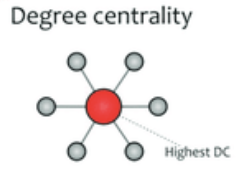
\includegraphics[width=\textwidth]{Degree.png}
    \caption{Degree Centrality}
    \label{fig:image1}
\end{subfigure}
\hfill
\begin{subfigure}[b]{0.35\textwidth}
    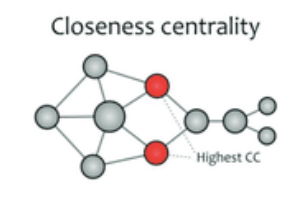
\includegraphics[width=\textwidth]{Closeness.png}
    \caption{Closeness Centrality}
    \label{fig:image2}
\end{subfigure}
\caption{Centrality}
\label{fig:doubleimage}
\end{figure}

\textbf{Community Detection} : A method to help in identifying groups of nodes that are more densely connected to each other than to the rest of the network \cite{albert2019a}. In this proposed research, we will use the Louvain algorithm and Label Propagation Algorithm (LPA). Louvain is chosen as it is a popular method for detecting communities in large networks based on modularity optimization, while LPA is relatively fast and scalable and able to gain insights early. They both can efficiently reveal the high-level compartmentalization of the network, showing how investor-startup clusters form. To better visualize community detection, please take a look into Figure 3 below.

\begin{figure}[h]
\centering
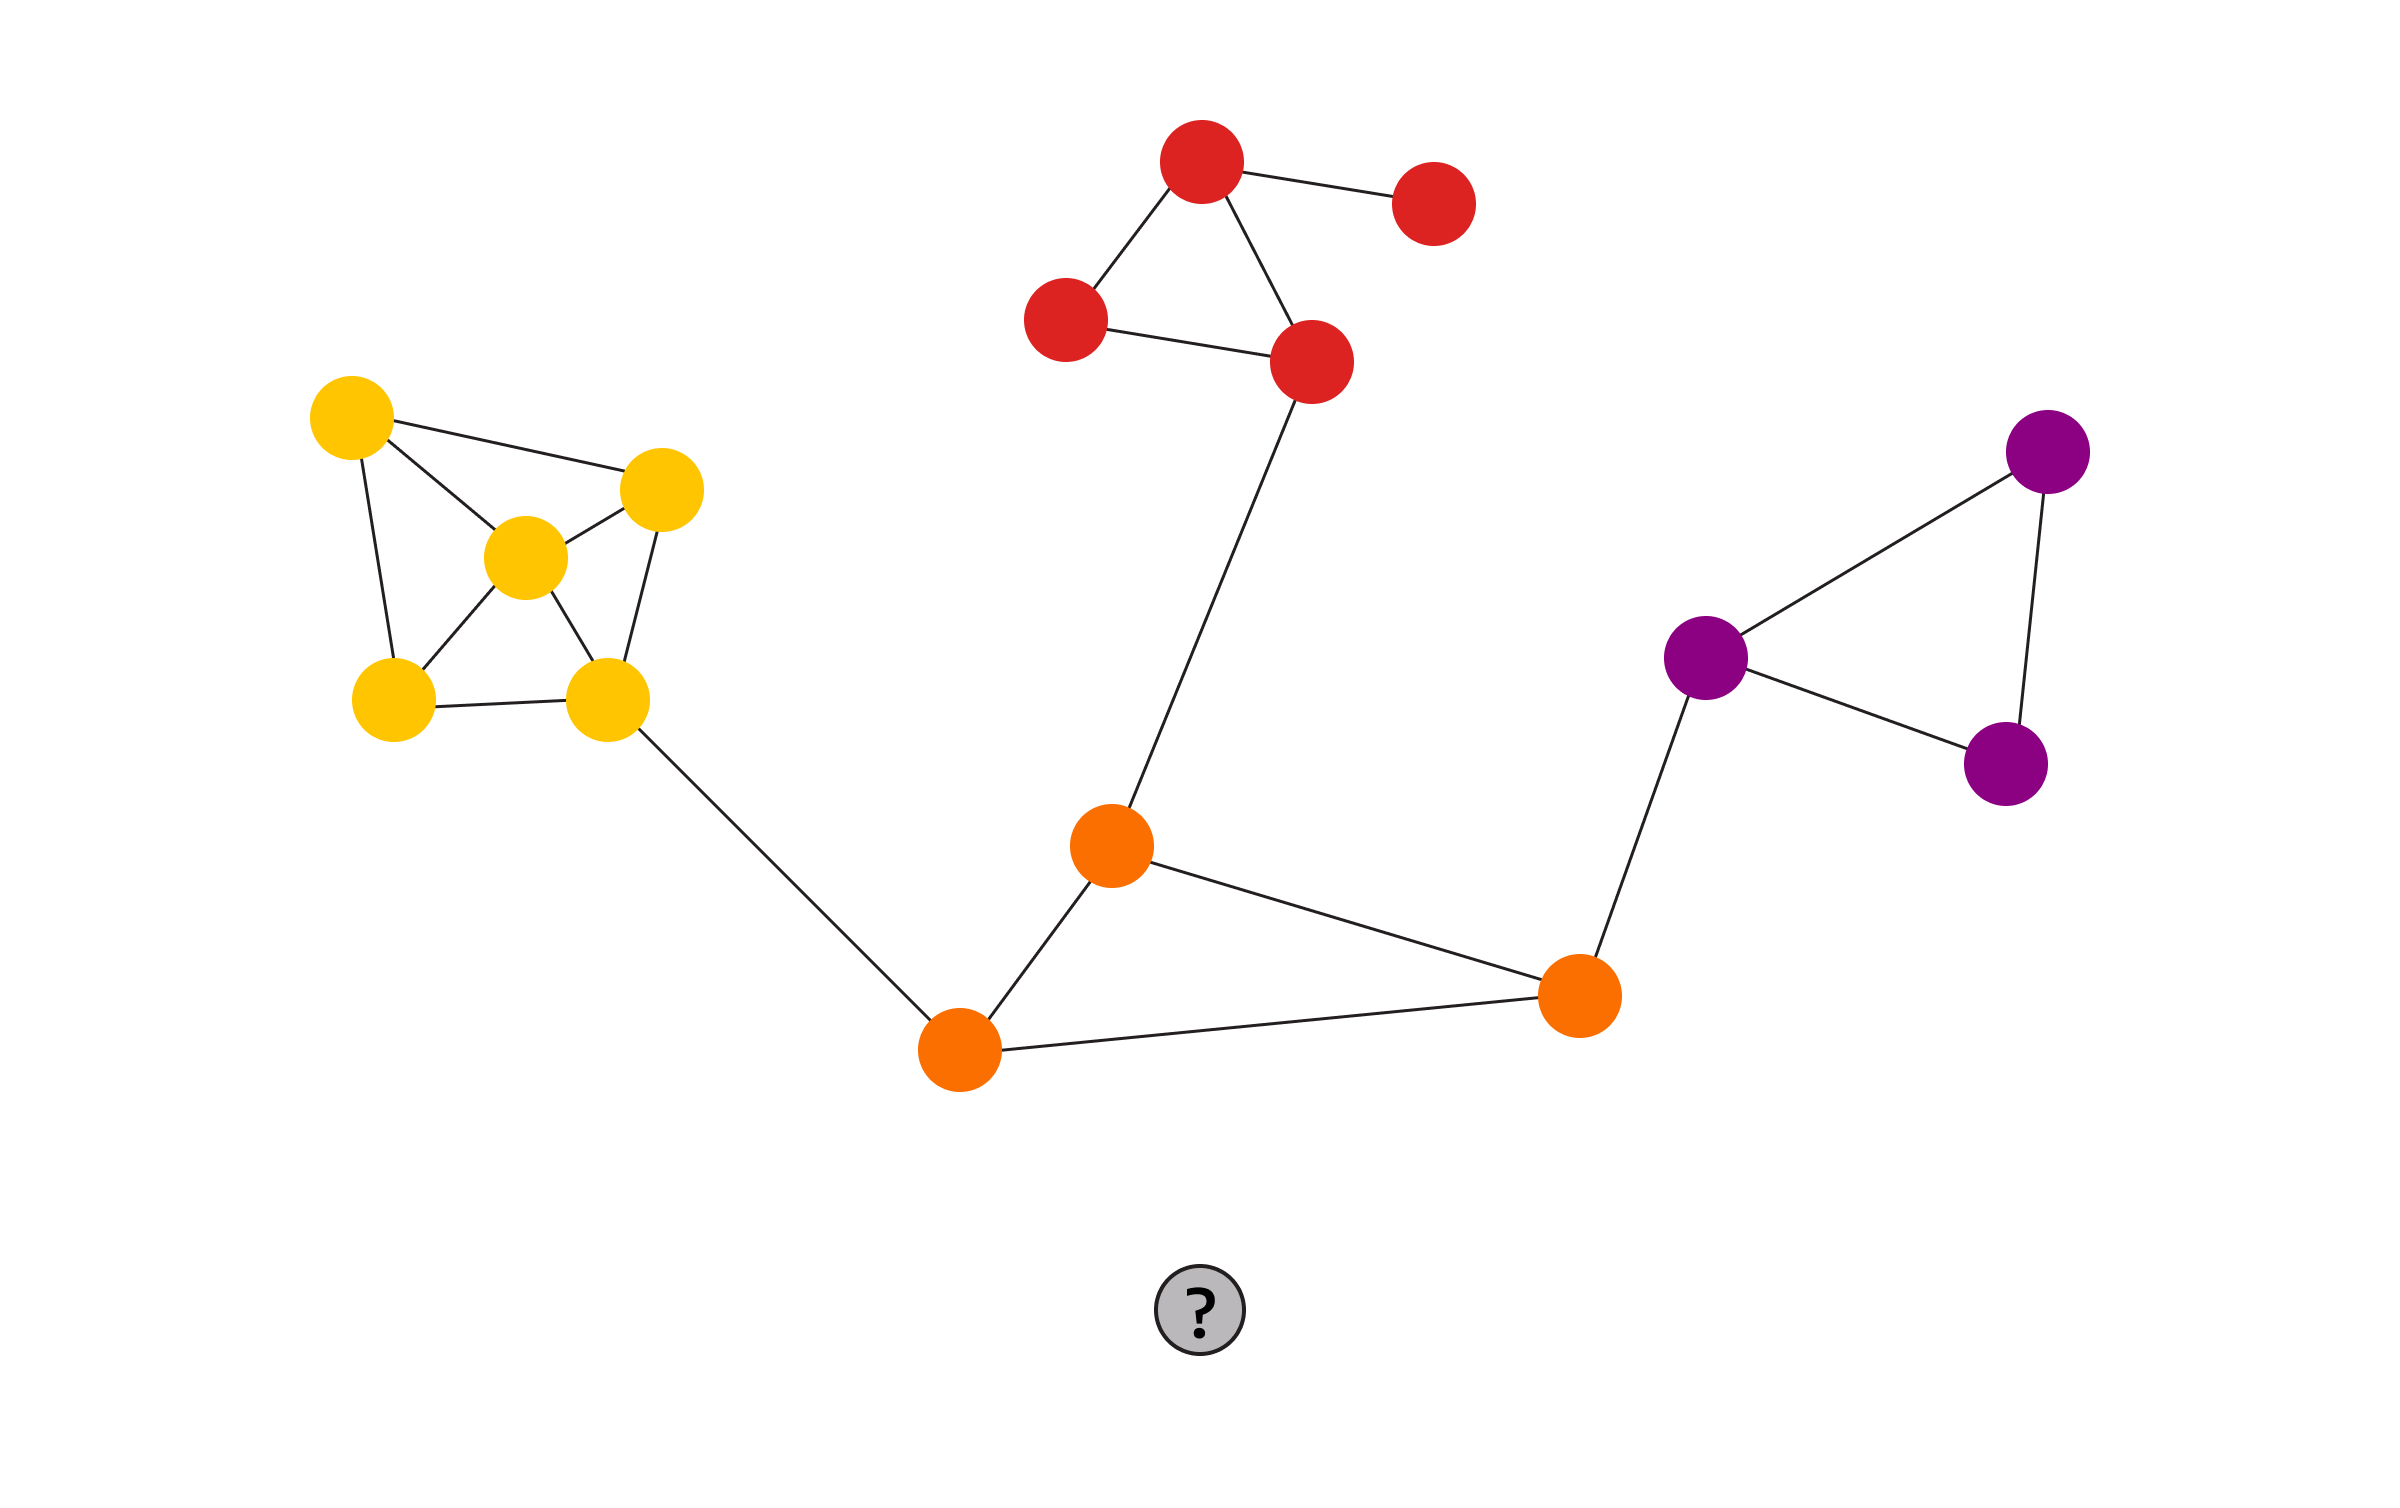
\includegraphics[width=0.4\textwidth]{community.png}
\caption{Community Detection}
\end{figure}

This research builds upon existing methodologies in startup success prediction, which have predominantly utilized machine learning techniques \cite{krishna2016a} \cite{sharchilev2018a}, hybrid network science and machine learning techniques \cite{carniel2023a} \cite{yang2020a}, agent-based modeling simulating market scenarios \cite{lengyel2020a}, and qualitative analysis based on case studies \cite{mccarthy2023a}. These approaches, while insightful, often overlook the distinct roles within networks, such as the specific dynamics between investors and startups, and generally lack the empirical grounding in actual investment data that our proposed bipartite network analysis provides.

This research proposal marks a significant departure from these existing approaches by focusing solely on the bipartite network analysis of investors and startups. Unlike previous works, which often revolve around characteristics like employee roles and interactions within companies, our approach emphasizes the dynamics between investors and startups. This shift allows us to explore how investment patterns influence startup success, which is less examined in current literature. By analyzing how centrality within this investor-startup network correlates with outcomes, this research aims to unveil nuanced insights that have been under explored in traditional studies, potentially leading to more targeted and effective investment strategies in the startup ecosystem.

\section{Programme and Methodology}
The proposed research will employ a bipartite network analysis to examine the relationships between investors and startups. This methodology is chosen due to its ability to reflect the complex and dual-role dynamics within the startup ecosystem—investors not only provide capital but also bring knowledge and networks that are crucial for startup success. The research will involve constructing a network where nodes represent investors and startups, and edges represent investment relationships. This approach is similar with employee and startups network created by Bonaventura et al. \cite{bonaventura2020a} and investor and startups network created by Carniel et al. research \cite{carniel2023a}.

This research will focus on centrality analysis to identify key actors within the network whose influence and connectivity predict greater success rates for startups. We will also use community detection to uncover clusters within the network that represent closely knit investment circles, which may facilitate knowledge and resource sharing. Temporal analysis will also be used to observe how network structures evolve over time and how these changes influence startup outcomes. Each of these techniques will contribute to understanding different facets of the network's influence on startup success, providing a comprehensive toolkit for analysis that surpasses traditional financial metrics or employee-focused network analyses.

This research will extend beyond the current state of the art by integrating investor-startup dynamics explicitly in the network model and employing a combination of network science methodologies that have not been collectively applied to this particular domain. This will provide a new horizon of analysis on startup's growth and success.

This research will be managed using a combination of weekly meetings with supervisor to ensure the research objectives are met and can be completed in a timely manner. Research progress will also be tracked using project management software to ensure timely delivery of each work package.

While this approach is innovative, it does have several limitations.
The model’s predictive power might be constrained by unforeseen economic or market factors that are not captured by network dynamics. The model will also only approach the prediction from one lens of analysis only, which is investor and startup interactions and dynamics. By acknowledging and addressing these limitations, the research will strive to provide robust insights while clarifying the scope and applicability of its findings.

\subsection{Risk Assessment}
There are a few risks involved in this research. First is the availability and quality of necessary data. As we heavily rely on investor and startups data in Crunchbase, there are risks that the fetched data is incomplete or limited. This can be mitigated by subscribing to Crunchbase's Academic Research Access Program, as we gain access to more complete and updated data inside Crunchbase's database. Second is imbalance and biased data, such as over representation of certain types of investors or startups. To mitigate this risk, we will implement rigorous data cleaning processes to identify and make a conscious effort to include data from underrepresented groups within the startup ecosystem. This might mean focusing on startups led by underrepresented founders or investors from less dominant geographies to ensure a balanced view in the network analysis. Last risk is the amount of data to be processed. As we only have very limited time to conduct the research, we will be exposed to the inability to finish the research on time. To mitigate this risk, we will do pre-processing to filter out incomplete data and reduce the data by certain factors that match our computing ability while maintaining the original data proportion.

\subsection{Ethics}
As predicting startup success is a widely researched field which often use publicly available data, it is hard to envisage any ethical concerns with this research. We can confirm that Crunchbase's data is aggregated and distributed legally and in line with data protection laws. Additionally, while it is still possible that the result of this research can sharpen the existing bias in investor and startup industries toward under-represented group \cite{ewens2020a} \cite{cumming2007a}, our methodology includes robust measures to identify and mitigate such tendency thus promoting the behavior to shift away from such biases.


\section{Evaluation}
\subsection{Data Collection}
The primary method of data collection for this research involves utilizing the Crunchbase API, a comprehensive source of information about startups, including details about their investors, funding rounds, and other relevant data. This approach will allow for systematic and scalable data extraction, ensuring that we capture a broad and detailed dataset encompassing various aspects of the startup ecosystem. Specifically, we will extract data on:
\begin{itemize}
    \item Startups: Names, industry sectors, dates of establishment, funding histories, and current status (open deals, acquisitions, IPOs, etc.).
    \item Investors: Types (e.g., angel, venture capital), investment patterns, and network links to other investors and startups.
    \item Investment Transactions: Amounts, dates, and the sequence of funding rounds to trace the flow of capital within the network.
\end{itemize}

\subsection{Result Interpretation}
To analyze and interpret the results, the research will focus on startups classified as "open deals"; those that have not yet received funding, been acquired, or been listed on the stock exchange. By examining these startups, the study will aim to assess the predictive power of early-stage network metrics, specifically centrality and community structure, on long-term economic performance.

Generally, it will follow these five steps : 
\begin{itemize}
    \item Using the collected data, we will construct a network where nodes represent startups and investors, and edges represent investment relationships. The network will be analyzed over time to capture the dynamics of investor influence and startup development
    \item Calculate centrality measures for each startup in the network. This analysis will identify startups that, at an early stage, are centrally positioned within the investor network, hypothesizing that these startups are more likely to succeed
    \item Apply algorithms to detect communities within the network, assuming that startups within highly interconnected investor communities may have better access to resources and knowledge, contributing to their success
    \item Analyze startups' success based on whether, within a 7-year window from founding, startups achieve significant milestones such as acquiring other firms, being acquired, or completing an IPO. This is similar as Bonaventura et al. approach \cite{bonaventura2020a}
    \item Compare the early predictions based on network centrality and community detection with actual outcomes to evaluate the accuracy and predictive power of these network metrics
\end{itemize}

\section{Expected Outcomes}
We expect that this research will produce similar results as Bonaventura et al. research \cite{bonaventura2020a}. While Bonaventura et al. focus on the knowledge transfer between startups as they key to startup's growth and success represented by employee movement, our research will show the similar knowledge transfer represented by investors network. We anticipate that by analyzing network centrality and community affiliations within this network, they can be robust predictors of startup growth and success and adding new dimension of data-driven decision making for startup investment on venture capital firms. Therefore, the result of this research will also prove Uzzi's theory about how social relations and networks benefit firms on navigating through challenges and striving \cite{uzzi2021a}.

\section{Research Plan, Milestones and Deliverables}

We propose to divide this research into three major stages. The first stage will be Crunchbase's API exploration to familiarize with Crunchbase's data and limitations. In this stage, we will also fetch the data and store it in our development environment. The next stage will be the development of the investor network, including all pre-process and data cleaning. The last stage will be the centrality and community detection analysis to prove the aforementioned theory's by Uzzi \cite{uzzi2021a} using similar parameters of startup's growth and success by Bonaventura et al. approach \cite{bonaventura2020a}. The detailed proposed timeline can be seen in Figure 4, while the milestones and deliverables are accessible in Table 1 and 2. The current update for this research is, we are currently in the first stage already and expect to finish stage 1 by the beginning of June 2024. We will proceed to further stages as this research proposal gets accepted in early June onward.

\definecolor{barblue}{RGB}{153,204,254}
\definecolor{groupblue}{RGB}{51,102,254}
\definecolor{linkred}{RGB}{165,0,33} 

\begin{figure}[htbp]
\begin{ganttchart}[
    y unit title=0.4cm,
    y unit chart=0.5cm,
    vgrid,hgrid,
    x unit=1.55mm,
    time slot format=isodate,
    title/.append style={draw=none, fill=barblue},
    title label font=\sffamily\bfseries\color{white},
    title label node/.append style={below=-1.6ex},
    title left shift=.05,
    title right shift=-.05,
    title height=1,
    bar/.append style={draw=none, fill=groupblue},
    bar height=.6,
    bar label font=\normalsize\color{black!50},
    group right shift=0,
    group top shift=.6,
    group height=.3,
    group peaks height=.2,
    bar incomplete/.append style={fill=green}
   ]{2024-06-01}{2024-08-16}
   \gantttitlecalendar{month=name}\\
   \ganttbar[
    progress=30,
    bar progress label font=\small\color{barblue},
    bar progress label node/.append style={right=4pt},
    bar label font=\normalsize\color{barblue},
    name=pp
   ]{API  exploration}{2024-06-01}{2024-06-07} \\
\ganttset{progress label text={}, link/.style={black, -to}}
\ganttgroup{Network Dev}{2024-06-07}{2024-06-28} \\
\ganttbar[progress=0, name=T1A]{Data Preprocess}{2024-06-07}{2024-06-21} \\
\ganttlinkedbar[progress=0]{Network Creation}{2024-06-21}{2024-06-28} \\
\ganttgroup{Network Analysis}{2024-06-28}{2024-07-21} \\
\ganttbar[progress=0, name=T2A]{Centrality Analysis}{2024-06-28}{2024-07-07} \\
\ganttlinkedbar[progress=0]{Community Analysis}{2024-07-08}{2024-07-21} \\
\ganttgroup{Dissertation}{2024-07-14}{2024-08-16} \\
  \ganttbar[progress=0]{Write up}{2024-07-14}{2024-08-16}
  \ganttset{link/.style={green}}
  \ganttlink[link mid=.4]{pp}{T1A}
  \ganttlink[link mid=.159]{pp}{T2A}
\end{ganttchart}
\caption{Gantt Chart of the activities defined for this research.}
\label{fig:gantt}
\end{figure}

\begin{table}[htbp]
    \begin{center}
        \begin{tabular}{|c|c|l|}
        \hline
        \textbf{Milestone} & \textbf{Week} & \textbf{Description} \\
        \hline
        $M_1$ & 1 & Feasibility study completed and data needed is fetched \\
        $M_2$ & 3 & Data is clean, complete, and scaled down \\
        $M_3$ & 4 & First prototype of network implementation completed \\
        $M_3$ & 7 & Evaluation completed for both centrality and community detection \\
        $M_4$ & 10 & Submission of dissertation \\
        \hline
        \end{tabular} 
    \end{center}
    \caption{Milestones defined in this research.}
    \label{fig:milestones}
\end{table}

\begin{table}[htbp]
    \begin{center}
        \begin{tabular}{|c|c|l|}
        \hline
        \textbf{Deliverable} & \textbf{Week} & \textbf{Description} \\
        \hline
        $D_1$ & 7 & Implementation of investor network \\
        $D_2$ & 8 & Evaluation report on the network \\
        $D_3$ & 10 & Dissertation \\
        \hline
        \end{tabular} 
    \end{center}
    \caption{List of deliverables defined in this research.}
    \label{fig:deliverables}
\end{table}


%                Now build the reference list
\bibliographystyle{unsrt}   % The reference style
%                This is plain and unsorted, so in the order
%                they appear in the document.

{\small
\bibliography{main}       % bib file(s).
}
\end{document}

